% Created by tikzDevice version 0.12.3.1 on 2021-12-03 16:19:31
% !TEX encoding = UTF-8 Unicode
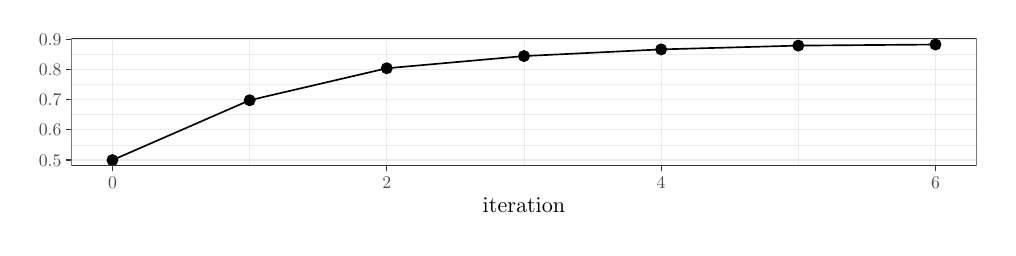
\begin{tikzpicture}[x=1pt,y=1pt]
\definecolor{fillColor}{RGB}{255,255,255}
\path[use as bounding box,fill=fillColor,fill opacity=0.00] (0,0) rectangle (346.90, 72.27);
\begin{scope}
\path[clip] (  0.00,  0.00) rectangle (346.90, 72.27);
\definecolor{drawColor}{RGB}{255,255,255}
\definecolor{fillColor}{RGB}{255,255,255}

\path[draw=drawColor,line width= 0.4pt,line join=round,line cap=round,fill=fillColor] (  0.00,  0.00) rectangle (346.90, 72.27);
\end{scope}
\begin{scope}
\path[clip] ( 15.78, 22.32) rectangle (342.90, 68.27);
\definecolor{fillColor}{RGB}{255,255,255}

\path[fill=fillColor] ( 15.78, 22.32) rectangle (342.90, 68.27);
\definecolor{drawColor}{gray}{0.92}

\path[draw=drawColor,line width= 0.2pt,line join=round] ( 15.78, 29.92) --
	(342.90, 29.92);

\path[draw=drawColor,line width= 0.2pt,line join=round] ( 15.78, 40.83) --
	(342.90, 40.83);

\path[draw=drawColor,line width= 0.2pt,line join=round] ( 15.78, 51.74) --
	(342.90, 51.74);

\path[draw=drawColor,line width= 0.2pt,line join=round] ( 15.78, 62.65) --
	(342.90, 62.65);

\path[draw=drawColor,line width= 0.2pt,line join=round] ( 80.21, 22.32) --
	( 80.21, 68.27);

\path[draw=drawColor,line width= 0.2pt,line join=round] (179.34, 22.32) --
	(179.34, 68.27);

\path[draw=drawColor,line width= 0.2pt,line join=round] (278.46, 22.32) --
	(278.46, 68.27);

\path[draw=drawColor,line width= 0.4pt,line join=round] ( 15.78, 24.46) --
	(342.90, 24.46);

\path[draw=drawColor,line width= 0.4pt,line join=round] ( 15.78, 35.37) --
	(342.90, 35.37);

\path[draw=drawColor,line width= 0.4pt,line join=round] ( 15.78, 46.28) --
	(342.90, 46.28);

\path[draw=drawColor,line width= 0.4pt,line join=round] ( 15.78, 57.19) --
	(342.90, 57.19);

\path[draw=drawColor,line width= 0.4pt,line join=round] ( 15.78, 68.10) --
	(342.90, 68.10);

\path[draw=drawColor,line width= 0.4pt,line join=round] ( 30.64, 22.32) --
	( 30.64, 68.27);

\path[draw=drawColor,line width= 0.4pt,line join=round] (129.77, 22.32) --
	(129.77, 68.27);

\path[draw=drawColor,line width= 0.4pt,line join=round] (228.90, 22.32) --
	(228.90, 68.27);

\path[draw=drawColor,line width= 0.4pt,line join=round] (328.03, 22.32) --
	(328.03, 68.27);
\definecolor{drawColor}{RGB}{0,0,0}

\path[draw=drawColor,line width= 0.6pt,line join=round] ( 30.64, 24.41) --
	( 80.21, 46.04) --
	(129.77, 57.60) --
	(179.34, 62.01) --
	(228.90, 64.42) --
	(278.46, 65.79) --
	(328.03, 66.18);
\definecolor{fillColor}{RGB}{0,0,0}

\path[draw=drawColor,line width= 0.4pt,line join=round,line cap=round,fill=fillColor] ( 30.64, 24.41) circle (  1.96);

\path[draw=drawColor,line width= 0.4pt,line join=round,line cap=round,fill=fillColor] ( 80.21, 46.04) circle (  1.96);

\path[draw=drawColor,line width= 0.4pt,line join=round,line cap=round,fill=fillColor] (129.77, 57.60) circle (  1.96);

\path[draw=drawColor,line width= 0.4pt,line join=round,line cap=round,fill=fillColor] (179.34, 62.01) circle (  1.96);

\path[draw=drawColor,line width= 0.4pt,line join=round,line cap=round,fill=fillColor] (228.90, 64.42) circle (  1.96);

\path[draw=drawColor,line width= 0.4pt,line join=round,line cap=round,fill=fillColor] (278.46, 65.79) circle (  1.96);

\path[draw=drawColor,line width= 0.4pt,line join=round,line cap=round,fill=fillColor] (328.03, 66.18) circle (  1.96);
\definecolor{drawColor}{gray}{0.20}

\path[draw=drawColor,line width= 0.4pt,line join=round,line cap=round] ( 15.78, 22.32) rectangle (342.90, 68.27);
\end{scope}
\begin{scope}
\path[clip] (  0.00,  0.00) rectangle (346.90, 72.27);
\definecolor{drawColor}{gray}{0.30}

\node[text=drawColor,anchor=base east,inner sep=0pt, outer sep=0pt, scale=  0.64] at ( 12.18, 22.26) {0.5};

\node[text=drawColor,anchor=base east,inner sep=0pt, outer sep=0pt, scale=  0.64] at ( 12.18, 33.17) {0.6};

\node[text=drawColor,anchor=base east,inner sep=0pt, outer sep=0pt, scale=  0.64] at ( 12.18, 44.08) {0.7};

\node[text=drawColor,anchor=base east,inner sep=0pt, outer sep=0pt, scale=  0.64] at ( 12.18, 54.99) {0.8};

\node[text=drawColor,anchor=base east,inner sep=0pt, outer sep=0pt, scale=  0.64] at ( 12.18, 65.90) {0.9};
\end{scope}
\begin{scope}
\path[clip] (  0.00,  0.00) rectangle (346.90, 72.27);
\definecolor{drawColor}{gray}{0.20}

\path[draw=drawColor,line width= 0.4pt,line join=round] ( 13.78, 24.46) --
	( 15.78, 24.46);

\path[draw=drawColor,line width= 0.4pt,line join=round] ( 13.78, 35.37) --
	( 15.78, 35.37);

\path[draw=drawColor,line width= 0.4pt,line join=round] ( 13.78, 46.28) --
	( 15.78, 46.28);

\path[draw=drawColor,line width= 0.4pt,line join=round] ( 13.78, 57.19) --
	( 15.78, 57.19);

\path[draw=drawColor,line width= 0.4pt,line join=round] ( 13.78, 68.10) --
	( 15.78, 68.10);
\end{scope}
\begin{scope}
\path[clip] (  0.00,  0.00) rectangle (346.90, 72.27);
\definecolor{drawColor}{gray}{0.20}

\path[draw=drawColor,line width= 0.4pt,line join=round] ( 30.64, 20.32) --
	( 30.64, 22.32);

\path[draw=drawColor,line width= 0.4pt,line join=round] (129.77, 20.32) --
	(129.77, 22.32);

\path[draw=drawColor,line width= 0.4pt,line join=round] (228.90, 20.32) --
	(228.90, 22.32);

\path[draw=drawColor,line width= 0.4pt,line join=round] (328.03, 20.32) --
	(328.03, 22.32);
\end{scope}
\begin{scope}
\path[clip] (  0.00,  0.00) rectangle (346.90, 72.27);
\definecolor{drawColor}{gray}{0.30}

\node[text=drawColor,anchor=base,inner sep=0pt, outer sep=0pt, scale=  0.64] at ( 30.64, 14.31) {0};

\node[text=drawColor,anchor=base,inner sep=0pt, outer sep=0pt, scale=  0.64] at (129.77, 14.31) {2};

\node[text=drawColor,anchor=base,inner sep=0pt, outer sep=0pt, scale=  0.64] at (228.90, 14.31) {4};

\node[text=drawColor,anchor=base,inner sep=0pt, outer sep=0pt, scale=  0.64] at (328.03, 14.31) {6};
\end{scope}
\begin{scope}
\path[clip] (  0.00,  0.00) rectangle (346.90, 72.27);
\definecolor{drawColor}{RGB}{0,0,0}

\node[text=drawColor,anchor=base,inner sep=0pt, outer sep=0pt, scale=  0.80] at (179.34,  5.56) {iteration};
\end{scope}
\end{tikzpicture}
